\chapter{Theoretical Aspects}

Regarding the theoretical aspects of the current paper, we present the following concepts:
\section{Neuronal Network}
The preliminary principle of a \textit{neuron} consists in a set of \weights{weights} and a set of \textit{biases}.
\textit{Weights} are a set of numerical values (initially arbirtrary) which throughout the passing
of the input through the Neural Network will be transformed and later, at the end of the training
process will be saved (basically representing the \texit{model}).
\textit{Biases}, similar to the intercept of a linear equation, represent aditional parameters to the network whose
purpose is to adjust the output of the weighted sum of the input.

\begin{center}
	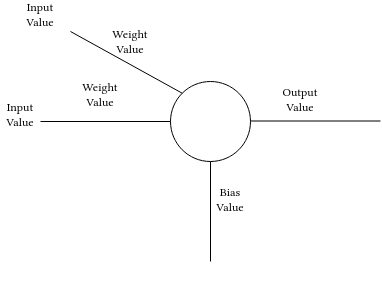
\includegraphics[width = 4.2in]{images/genericneuron.png}
	\centerline{\captionof{Figure 3.1: }{Illustration of a generic neuron}}
\label{neuron}
\end{center}

A Neuronal Network is a set of \textit{neurons} (as previously defined), grouped in \textit{layers},
during the traversal of which the process of learning takes place.
Depending on the type of layers as well as their configuration multiple various operations regarding the input feeded take
place.

\begin{center}
	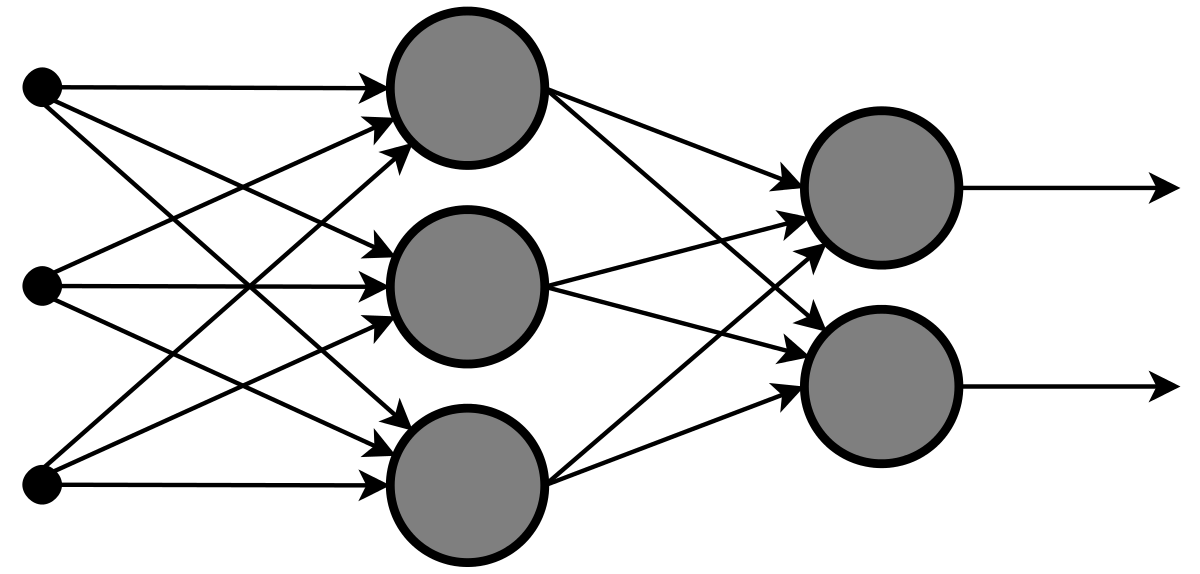
\includegraphics[width = 4.2in]{images/genericnn.png}
	\centerline{\captionof{Figure 3.2: }{Illustration of a generic neural network (Image source \cite{gennn}) }}
\label{nn}
\end{center}


\section{Layers}

As seen before, a layer is a set of neurons, which is described by an input (having a specific shape)
and an output with a shape resulted from the specific calculations.

Throught a Neural Network architecture we may find multiple types of layers such as: Fully connected layer(\textit{Dense
} layers), \textit{Flattening} layers, \textit{2D Convolutional } layers, \textit{Batch Normalization} layers etc.
Of these aforementioned layers, we will go into the specifics of \textit{Batch Normalization}.
\subsection*{Batch Normalization}
A \textit{batch} of data is a subset of the training data with a fixed size.
Normalization is a technique which involves mapping a given set of values to a new one, preserving its value ratios.


BatchNormalization is a technique for standardizing the inputs recieved from the previous layer,
with the effect of stabilizing the learning process and reduce
the number of training epochs required.
The BatchNormalization layer works by applying a linear scale and then shift the
result of the batch, following the formula:

\begin{center}
	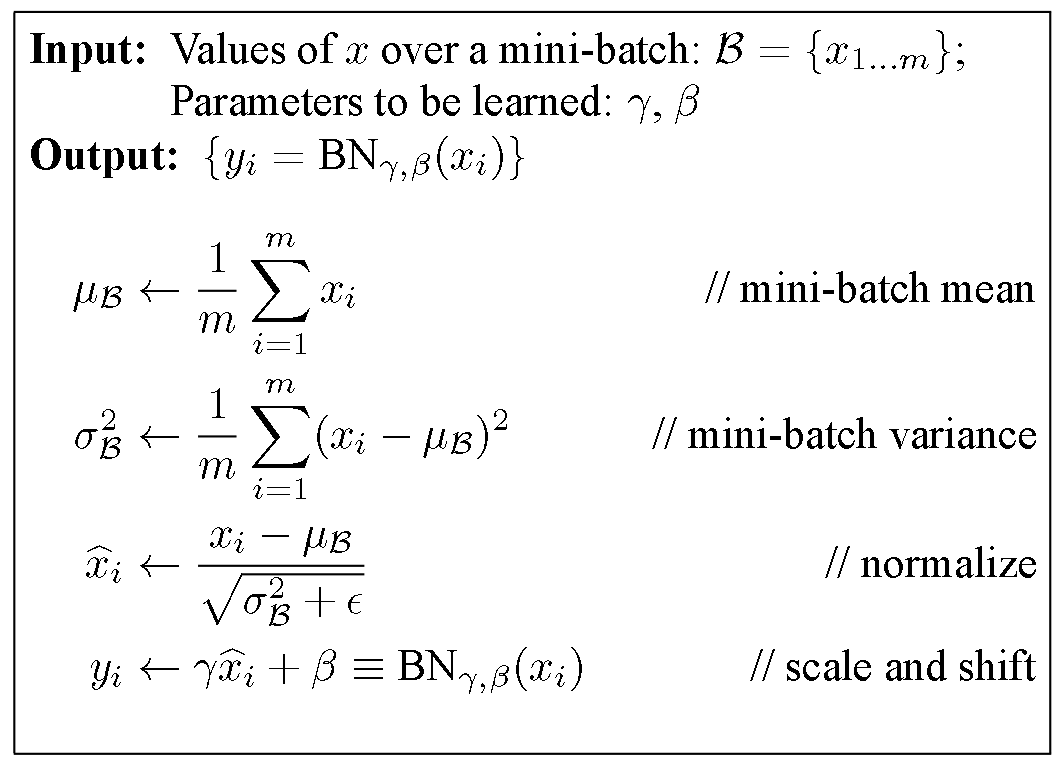
\includegraphics[width = 4.2in]{images/bn.png}
	\centerline{\captionof{Figure 3.3: }{The Batch Normalization formula(Image source \cite{bn}) }}
\label{bn}
\end{center}
The Batch Normalization layer formula is composed of three components:
\begin{itemize}
	\item gamma: The layer scaling factor.
	\item \^x} : The output of the normalization process, computed by substracting a batch element by the
		mean of the whole batch and then divide the output by the standard variation
		of the batch.
	\item beta: The layer shifting factor.
\end{itemize}


\section{Activation Functions}
The activation function is a function added to a layer which enables the Neural Network to
fit nonlinear problems.
The activation functions fall into 2 categories:
\begin{itemize}
	\item Linear(e.g. ReLU) which emulates the \textit{firing} of a neuron by checking whether or not the
		function output is below a critical value.
	\item Non-Linear(e.g. Sigmoid) used most of the times as an activation function for the last layer, because it normalizes the values given between 0 and 1, thus producing an informative output in regards to the confidence of the model prediction.
\end{itemize}
We will now discuss the \textit{Rectified Linear Unit(ReLU)} function:
\subsection*{Rectified Linear Unit(ReLU)}
\textit{ReLU} is an activation function which clips negative input values using the formula ilustrated below. Among the
advantages of the ReLU function we mention the simplicity of the computation and the fact that ReLU prevents the
\textit{vanishing gradient problem}(the invalidation of the neuron values during backpropagation due to the derivation
process).
\begin{center}
	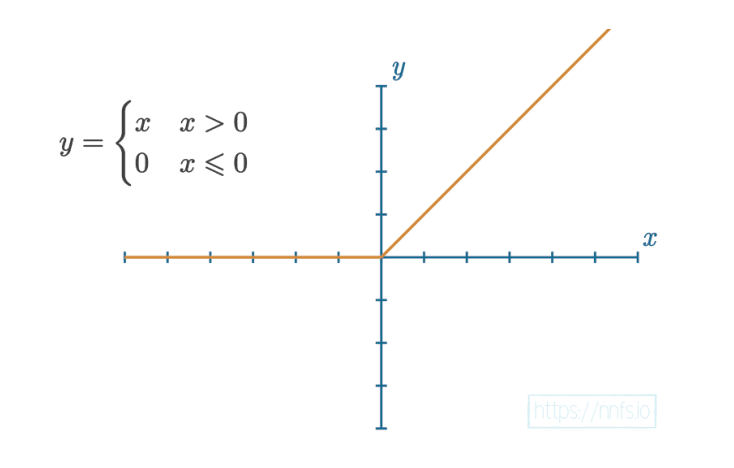
\includegraphics[width = 4.2in]{images/relu.png}
	\centerline{\captionof{Figure 3.4: }{The ReLU formula and graphic illustration(Image source \cite{nnfs}) }}
\label{relu}
\end{center}
\section{Optimizers}
Optimizers are algorithms used to improve the parameters of a given neural network (such as weights and biases)
in order to reduce the \textit{model loss value}.
Depending on the type of the problem to solve we can choose from multiple optimizers such as SGD
(Stochastic Gradient Descent), RMSProp (Root Mean Squared Error Propagation), Adagarad(Adaptive Gradient Algorithm) etc.

\subsection*{Stochastic Gradient Descent(SGD)}
The SGD optimizers works by slicing a batch of data into individual inputs then updating the
weights and biases of a layer by substracting the product of the \textit{learning rate}( a parameter that controls the rate
at which a model changes) and the backpropagation output.

\section{Metrics}
The metrics function provide the means for analyzing and interpreting the performance of a Neural Network.
The two most utilised metrics in Neural Network analysis are:
\begin{itemize}
	\item \textit{Loss}:
		the cost function of the network with the main goal of computing
		the incorrectness of the model prediction . Common loss functions include \textit{Cross-Entropy Loss},
		\textit{Categorical Cross-Entropy}, \textit{Mean Square Error}.
	\item \textit{Accuracy}: is a metric for evaluation of the model classification,
		computed by dividing the number of correct predictions by the total
		number of predictions.
		The accuracy is the most "human readable" metric, illustrating the
		performance of the model in terms of sucessful predictions. Amongst the accuracy
		functions we recall the \textit{Categorical Accuracy} and \textit{Regression Accuracy}.
\end{itemize}

In order to accuracy as well as other realted metrics (\textit{sensitivity,recall,precision}) we defined the following
notations:
\begin{center}
	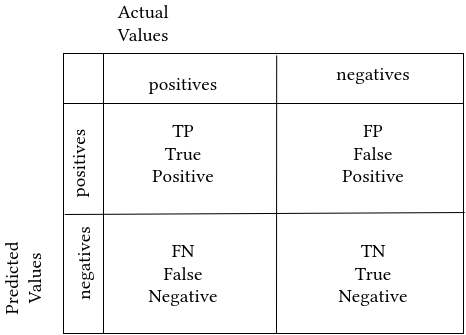
\includegraphics[width = 4.2in]{images/cm.png}
	\centerline{\captionof{Figure 3.5: Confusion matrix.}}
\label{cm}
\end{center}
Thus we compute the accuracy using the following formula:
\[accuracy = \frac{TP+TN}{TP+FN+FP+TN} \]
